\section*{Acknowledgments}
To Be Completed. Currently this will serve as a to-do list:

input list of figures

input list of tables
\iffalse

Acknowledgement should be given to the MIT Milner Hadronic Physics group: Richard Milner, Douglas Hasell, Igor Korover, Xiaqing Li, Patrick Moran, Sangbaek Lee, and Robert Johnston. This work was also facilitated by the use of OSG and MIT Tier 2 computing, so we would like to thank Maurizio Ungaro, Christoph Paus, Ernie Ihloff, Jim Kelsey, and others for their technical support. 


I'd like to take this chance to acknowledge \newline
\newline

\vspace{2cm}

\begin{flushright}
    absolutely nobody
\end{flushright}

\begin{figure}[hbt]
	\centering
	 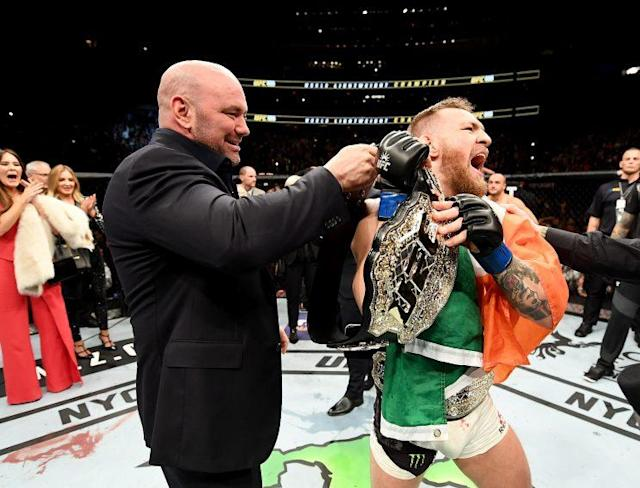
\includegraphics[trim={5cm 0 0 0.8cm} ,clip,width=.725995\textwidth]{templates/me.jpg}

\end{figure}

/joke
Lupe Fiasco, for inspiration, Nick Cambi for perspiration, and Inky Johnson for motivation.

joe jack Cathy Karen Dow (mit general services)
Ernie Kelsey
Tami
Messina
Rice
Miskimen
Joe (service guy from UMass)
All JLab hockey guys
Elton Smith JLab
the tech guy from JLab that was fat and crazy
Thesis Peter Charles axel Fabian jlab people
Fridericke Jentoft
Jan, ross, frank taylor for thesis

I'd like to take this chance to acknowledge


\graphicspath{ {./images/} }

The universe is immense and it seems to be homogeneous, 
in a large scale, everywhere we look at.



\begin{figure}[hbt]
	\centering
	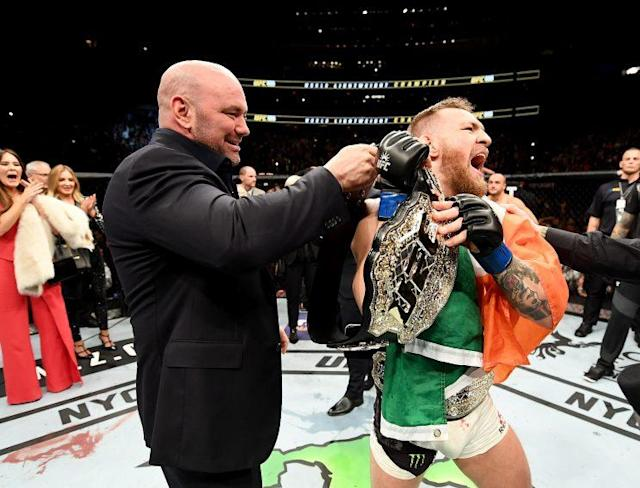
\includegraphics{templates/me.jpg}
\end{figure}


absolutely nobody


\fi
